%% Autores:
%%      lcabrera
%%      li-po
%%      mojopikon

%% Versión
%% $Id$

%% Algunas aplicaciones a detallar:
%% gnotepad,acroread, ghostview, gnumeric, gqview, videolan client, xine

%iCorrecam: 2
%mojopikon: 2
%li-po: 9

\chapter{Aplicaciones diversas} 
\label{aplicaciones.tex}
\index{Aplicaciones}

En  este  apartado  trataremos,  de manera  muy  superficial,  algunas
aplicaciones de uso cotidiano en Linux.

%% Primera  sección
\section{Aplicaciones Gráficas} 

Las aplicaciones gráficas disponibles hoy día cubren un amplio abanico
de actividades. Aquí expondremos sólo algunas pocas de ellas.

\subsection{Internet}
\index{Aplicaciones!Internet}

Dentro  de las  diversas  aplicaciones relacionadas  con Internet  que
podemos usar  a diario,  podemos resaltar  aquellas que  se encuentran
orientadas a la  comunicación directa entre personas, como  lo son los
programas de Mensajería Instantanea o los clientes de IRC

\subsubsection*{Gaim}
\index{Aplicaciones!Gaim}

Entre  la   surtida  gama  de  clientes   de  Mensajería  Instántanea,
destacaremos el programa {\sf Gaim}. La característica que nos mueve a
destacar este programa en particular es la gran cantidad de protocolos
soportados  en  un  único  cliente. Con  este  cliente  de  Mensajería
Instántanea podremos conectarnos con los  servicios de {\sf MSN}, {\sf
Yahoo}, {\sf AOL}, {\sf ICQ}, {\sf  Jabber}, {\sf Napster} o el propio
IRC, por citar algunos de los protocolos soportados.

% Poner una captura del Gaim

\subsubsection*{XChat/KVirc}
\index{Aplicaciones!IRC}

Otro de los servicios que  se suelen utilizar con bastante frecuencia,
se encuentran las «consultas» al IRC. Este protocolo nos permite estar
interconectados  con  otros grupos  de  usuarios,  de una  manera  muy
dinámica.  En Linux,  en  el  apartado de  clientes  de IRC  gráficos,
destacan especialmente dos clientes: {\sf XChat} y {\sf KVirc}

{\sf  XChat} es  un  cliente  de IRC  muy  flexible,  que nos  permite
mantener sesiones no sólo en varios  canales al mismo tiempo, sino que
incluso nos  permite conectar  con varios servidores  de IRC  al mismo
tiempo, todo ello de una manera muy intuitiva.

% \begin{figure}[htbp]
% \centering
% 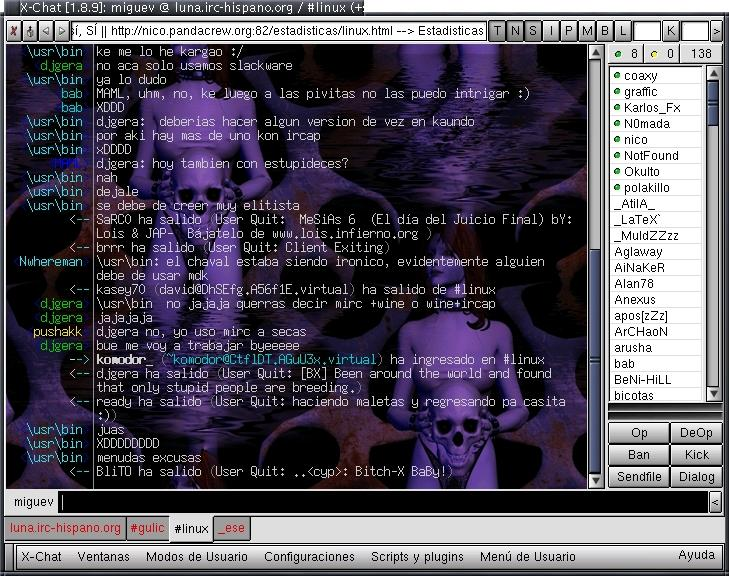
\includegraphics[width=\textwidth]{imagenes/xchat.eps}
% \caption{Cliente de IRC XChat}
% \end{figure}

De la  misma manera, el {\sf  KVirc} es otro cliente  gráfico capaz de
satisfacer al más exigente de  los usuarios. Entre otras cosas destaca
por las ayudas que presta a  aquellos que les gusta disfrutar haciendo
«scripts» para los clientes de IRC

\subsection{Multimedia}
\index{Aplicaciones!multimedia}

La reproducción  de los  diferentes formatos gráficos  es otro  de los
apartados que se suelen utilizar a  diario. Para los usuarios de otros
sistemas operativos  resulta normal el  poder disponer de  un software
capaz de  reproducir casi  cualquier fichero multimedia.  Sin embargo,
en  Linux ha  costado  un  gran esfuerzo  llegar  a  poder contar  con
reproductores como los que presentamos a continuación.

\subsubsection*{XMMS}
\index{Aplicaciones!XMMS}

{\sf XMMS (X  Multimedia System)} es el reproductor  multimedia de uso
general  en GNU/Linux.  Puede reproducir  cualquier formato  de audio,
tomándolo incluso de la red, y  algunos formatos de vídeo MPEG. Además
dispone  de  multitud  de  plugins:  efectos  visuales,  drivers  para
diferentes formatos  de entrada/salida,  y cosas tan  variopintas como
controlarlo mediante un  receptor de infrarojo casero  conectado en el
puerto serie de tu ordenador.

% \begin{figure}[hbtp]
% \centering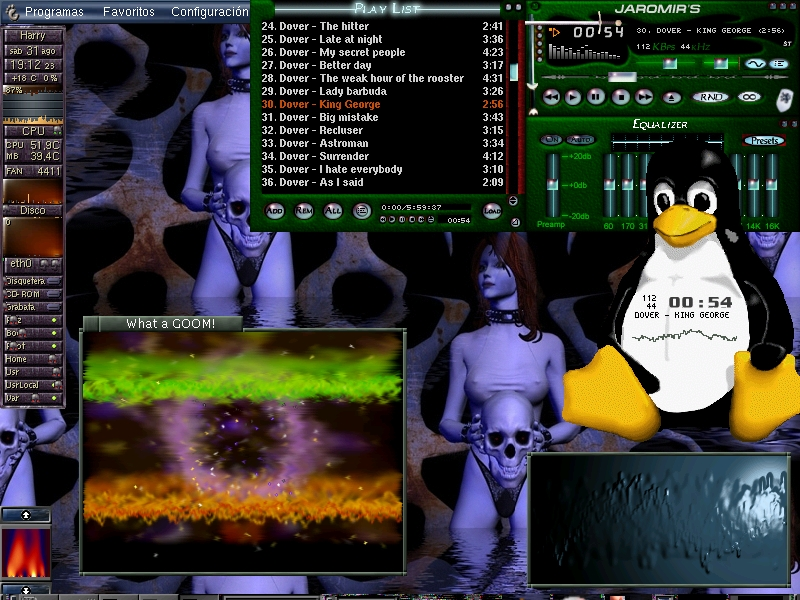
\includegraphics[width=\textwidth]{imagenes/xmms.eps}
% \caption{XMMS con varios plug-ins de visualización activados}
% \end{figure}

\subsubsection*{Xine}
\index{Aplicaciones!xine}

{\sf Xine} es el resultado de un esfuerzo continuado de superación por
parte  de  la  comunidad  que  lo desarrolla.  Cuando  se  comenzó  su
desarrollo, nadie esperaba  que alcanzara el nivel de  calidad del que
disfruta hoy día. Con {\sf Xine} puedes ver películas en formato MPEG,
ASF o DivX 5.

% \begin{figure}[hbtp]
% \centering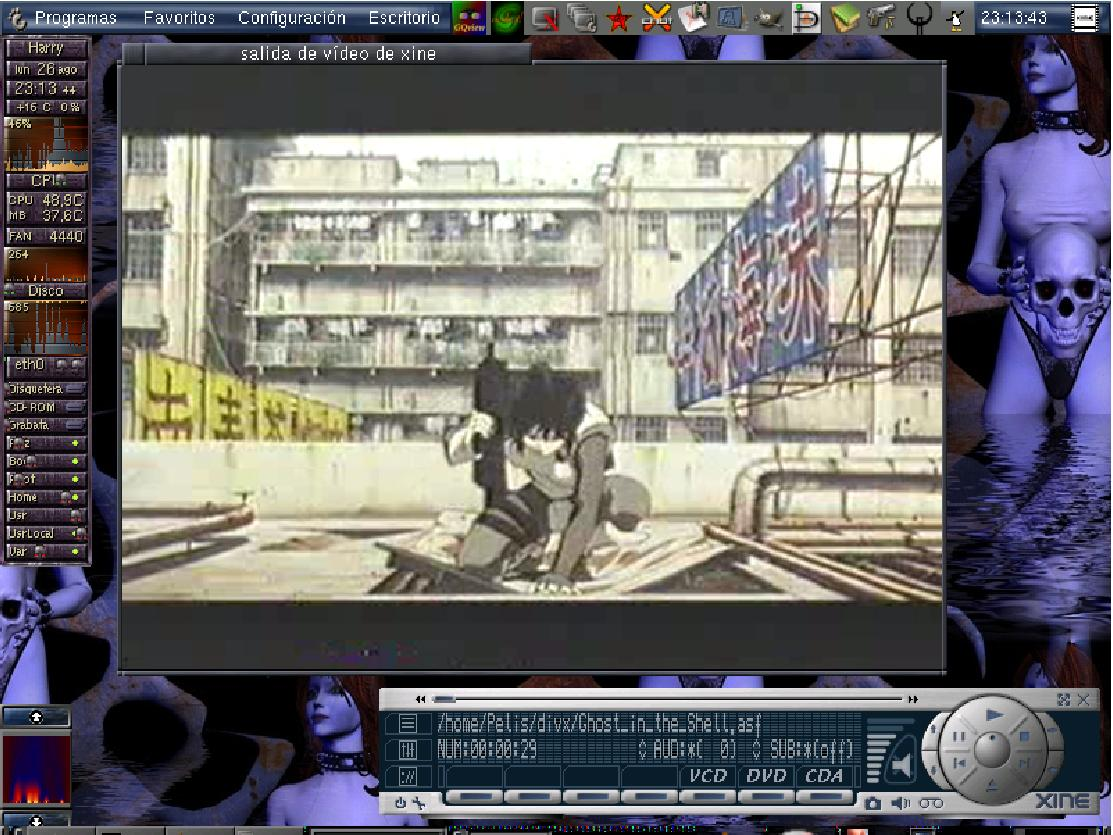
\includegraphics[width=\textwidth]{imagenes/xine.eps}
% \caption{Xine reproduciendo la película ``Ghost in the Shell''}
% \end{figure}

%\subsubsection*{Aviplay}

\subsubsection*{mpg321} 
\index{Aplicaciones!mpg321}
% <MojoPiKon> Me la pido :-)

{\tt mpg321} es  un reproductor de ficheros con formato  MP3. Se trata
de  un programa  de línea  de comandos  no interactivo,  esto es,  uno
ejecuta el programa con una serie de argumentos, y una vez el programa
comienza a  ejecutarse, no  existe interacción entre  el usuario  y el
programa, sino que  se limita a realizar las operaciones  que le hemos
proporcionado en la línea de comandos.

La forma  más asequible  para reproducir  MP3 con  {\tt mpg321}  es el
siguiente  comando, suponiendo  que nos  encontremos en  un directorio
que contenga ficheros MP3.

\begin{verbatim}
$ mpg321 *.mp3
\end{verbatim}

Para aquellos que no les basta esto, hay una amplia gama de parámetros
que pueden pasarse a {\tt mpg321}:

\begin{verbatim}
$ mpg321 -o tipo_de_dispositivo fichero_mp3
\end{verbatim}

\noindent donde tipo  de dispositivo puede ser oss, alsa,  esd, sun, o
arts.

Esto, que en principio no tiene  interés alguno para la mayor parte de
la  gente (pues  {\tt mpg321}  funcionará (en  la mayor  parte de  los
casos)  sin especificar  este  parámetro,  puede resultar  interesante
en  caso de  que,  por  ejemplo, queramos  reproducir  dos  o más  MP3
simultáneamente.

Si tenemos {\sf  artsd} instalado, podemos hacer  esto arrancando {\tt
mpg321} de la forma:

\begin{verbatim}
$ mpg321 -o arts fichero.mp3
\end{verbatim}

tras lo cual  podemos repetir la operación tantas  veces como queramos
en la misma o en diferentes consolas.

Este parámetro (-o) funciona conjuntamente con el siguiente:

\begin{verbatim}
$ mpg321 -a nombre_de_dispositivo fichero_mp3 
\end{verbatim}

\noindent donde  {\tt nombre\_de\_dispositivo}  es algo así  como {\tt
/dev/dsp}, {\tt  /dev/sound/dsp1}, o aquel que  utilice el dispositivo
de sonido que queramos utilizar para oir nuestros MP3 :-)

Utilización de listas de reproducción:

Podemos cargar una ``playlist'' de un  fichero TXT con las rutas a los
ficheros MP3 que queramos que la compongan. Esto se hace de la forma:

\begin{verbatim}
$ mpg321 -@ fichero.txt
\end{verbatim}

Reproducción aleatoria de ficheros:

Para esto  tenemos dos parámetros: -z  y -Z; {\tt -Z}  reproduce todos
los ficheros especificados  de forma aleatoria hasta  que paremos {\tt
mpg321}, {\tt -z} reproduce todos  los ficheros especificados de forma
aleatoria una sola vez.

Para  aquellos  que  crean  que   una  aplicación  no  interactiva  de
reproducción de MP3 puede  ser totalmente inútil, existen alternativas
en  modo  texto, como  {\tt  mp3blaster}  (también reproduce  ficheros
ogg-vorbis, el formato libre alternativo  al mp3, que por el contrario
está patentado y es propietario de Fraunhoffer).

Para el entorno {\sf X-Window}, tenemos {\sf XMMS}, que es un perfecto
clon de  {\sf Winamp},  el conocido reproductor  MP3 para  ese sistema
operativo que todos conocen.

\subsection{Ofimática}

Otra área compleja de abordar en su  momento, fue la de la creación de
un entorno ofimático del nivel adecuado al que ya gozaban los usuarios
de otros sistemas operativos. Esta  tarea aparecía como inabordable en
unos primeros  momentos, pero sólo era  una cuestión de tiempo  el que
«La  Comunidad» aportará  los recursos  adecuados para  conseguir este
tipo de  entornos. El resultado  es que  hoy día disponemos  de varias
alternativas  para poder  enfrentarnos a  la  dura tarea  de abrir  un
editor de  textos al más  puro estilo {\sf Word}  o abrir una  hoja de
cálculo similar al programa {\sf Excel}.

%\subsubsection*{Koffice}
% \subsubsection*{OpenOffice}
% \index{Aplicaciones!OpenOffice}

% {\sf OpenOffice} es, sin duda,  el proyecto más ambicioso, relacionado
% con  la ofimática,  que tenemos  en  marcha hoy  en día  dentro de  la
% comunidad de desarrolladores de Software Libre.

% {\sf OpenOffice} abarca  todo lo que se puede desear  dentro del campo
% de la ofimática de base, cubriendo sobradamente las necesidades reales
% de cualquier usuario de Linux dentro de una empresa. Como este tema ya
% se  trata  en el  tema  \ref{openoffice},  nos limitaremos  a  exponer
% algunas  capturas  de  pantalla  de los  diferentes  módulos  de  {\sf
% OpenOffice}.

%(Poner captura del Procesador de Textos)
%(Poner captura de la Hoja de Cálculo)
%(Poner captura del equivalente al PowerPoint)
%(Poner captura de la parte de acceso a Datos)
%(Poner otras capturas)


% \subsection{Gráficos}
% \index{Aplicaciones!Gráficos}
%\subsubsection*{Gimp}

%\subsubsection*{eog}

%\subsubsection*{gqview}

\subsubsection*{Ghostview}
\index{Aplicaciones!Ghostview}

{\sf  Ghostview}   es  una   interface  de   usuario  X11   para  {\sf
Ghostscript}, que  te permite ver  y navegar por  ficheros PostScript.
Hay diversos derivados de {\sf Ghostview} que son de uso frecuente:

{\sf  Gv} es  una  versión de  {\sf Ghostview}  con  una interface  de
usuario mejorado y con capacidad para abrir ficheros PDF.

{\sf MGv}  es un  front-end  basado en  Motif  para {\sf  Ghostscript}
{\sf basado en Ghostview 1.5}.

Hay un programa similar llamado  {\sf GSview} que está disponible para
usarlo bajo Linux/X11,  Windows y OS/2, pero no está  derivado de {\sf
Ghostview}.

Algunas características de {\sf Ghostview} son:

\begin{enumerate}

\item {\sf  Ghostview} analiza  todas las  versiones conocidas  de las
{\sf Convenciones de Estructuración de Documentos de Adobe}.

\item El tamaño de la página  se determina automáticamente a partir de
los comentarios de estructuración del documento.

\item El usuario puede anular los valores desde los comentarios.

\item El  tamaño de la  ventana se establece  en el cuadro  de límites
para los valores del PostScript Encapsulado.

\item El tamaño  por defecto de la página es  Letter y puede cambiarse
mediante {\tt Xresources} o en el  fichero de aplicación por defecto a
A4 (o a cualquier tamaño válido).

\item Las barras desplegables aparecen sólo cuando se necesitan.

\item La orientación  de la página se  determina automáticamente desde
los  comentarios de  estructuración  del documento.  El usuario  puede
ignorar los valores.

\item Capacidad para ver  en cuatro orientaciones: Vertical, apaisado,
inversa y apaisado a la derecha.

\item Capacidad para  restringir la presentación a escala  de grises o
monocromo (Requiere {\sf Ghostscript 2.6.1})

\item Capacidad para marcar páginas para imprimir o guardar.

\item Puede  mostrar ventanas de  zoom iguales  a la resolución  de la
impresora (1 punto mostrado = 1 punto de impresora).

\end{enumerate}

Aconsejamos poner  GNU {\sf Ghostscript 2.6.2}  que resuelve problemas
de versiones anteriores.

Una  vez  que  tengas  instalado {\sf  Ghostscript}  sólo  tienes  que
lanzarlo y  en {\tt  abrir documento}  poner la  ruta donde  tengas el
documento PostScript o PDF que quieras visualizar.

%\subsection{Desarrollo}

%\subsubsection*{Glade/Kdevelop}

%\subsubsection*{Cervicia/gcvs}

%\subsubsection*{Quanta/Bluefish}

\subsection{Editores}
\index{Aplicaciones!editores}

%\subsubsection*{AbiWord}

\subsubsection*{KWrite}
\index{Aplicaciones!KWrite}

{\sf KWrite} es un editor de texto para {\sf KDE 2.0}, pero también es
más que  un editor de  textos, pues es  un editor de  programación que
puede considerarse como  una alternativa parcial a  otros editores más
poderosos. Es  mejor usarlo  en combinación  con {\sf  Konqueror} como
visor de ficheros en distintos lenguajes.

Una de las principales características  de {\sf KWrite} es la sintaxis
coloreada, adaptada  para muchos lenguajes de  programación tales como
C/C++, Java, Python, Perl, Bash, Modula 2, HTML y Ada.

{\sf KWrite}  es muy  simple de  usar y cualquiera  que haya  usado un
editor de texto no tendrá problemas con él.

Arrastrar y  Pegar: {\sf KWrite}  usa el  protocolo de {\sf  KDE} para
Arrastre y  Pegado. Los ficheros  pueden ser arrastrados y  pegados en
{\sf KWrite} desde el Escritorio, {\sf Konqueror} o de cualquier sitio
de FTP abierto en una ventana de {\sf Konqueror}.

Opciones de líneas de comandos:  {\sf KWrite} puede iniciarse desde el
menú de  programas de {\sf KDE}  o desde el icono  del escritorio, así
como  desde la  línea  de  comandos de  un  terminal.  Hay unas  pocas
opciones útiles disponibles al hacer esto.

Especificar un fichero:  especificando la ubicación y el  nombre de un
fichero,  {\sf  KWrite} lo  abrirá  (o  lo creará)  inmediatamente  al
iniciarse. Esta opción sería algo similar a esto:

\begin{verbatim}
$ kwrite /home/midirectorio/docs/mifichero.txt
\end{verbatim}

Especificar un fichero desde Internet:  El método antes señalado puede
usarse  para abrir  ficheros de  Internet  (si se  tiene una  conexión
activa en ese momento). Por ejemplo:

\begin{verbatim}
$ kwrite ftp://ftp.kde.org/pub/kde/Welcome.msg
\end{verbatim}

Otras opciones de líneas de comando disponibles:

\begin{description}

\item[{\tt --help}] Lista  de las opciones más  básicas disponibles en
la línea de comandos.

\item[{\tt --help-qt}] Lista de  las opciones disponibles para cambiar
la forma en que {\sf KWrite} interactúa con {\sf Qt}.

\item[{\tt --help-kde}] Lista de las opciones disponibles para cambiar
la forma en que {\sf KWrite} interactúa con {\sf KDE}.

\item[{\tt  --help-all}]  Lista de  todas  las  opciones en  línea  de
comandos.

\item[{\tt  --author}] Lista  de los  autores  de {\sf  KWrite} en  la
ventana del terminal.

\item[{\tt --version}] Información  de la versión para  {\sf Qt}, {\sf
KDE} y {\sf KWrite}. También disponible con {\tt kwrite -V}

\end{description}

\paragraph{Teclas establecidas}

Muchas de las  teclas establecidas (atajos) pueden  configurarse en el
menú de especificaciones. Por defecto {\sf KWrite} trae las siguientes:

\begin{description}

\item[{\tt  Insert}]  Cambia  entre  el  modo de  Inserción  y  el  de
Sobreescribir.

\item[{\tt Flecha izquierda}] Mueve el cursor a la izquierda

\item[{\tt Flecha derecha}] Mueve el cursor a la derecha

\item[{\tt Flecha hacia arriba}] Mueve el cursor una línea haci arriba

\item[{\tt Flecha hacia abajo}] Mueve el cursor una línea hacia abajo

\item[{\tt Página adelante}] Mueve el cursor adelante una página

\item[{\tt Página atrás}] Mueve el cursor una página hacia atrás

\item[{\tt Retroceso}] Borra el carácter a la izquierda del cursor.

\item[{\tt Inicio}] Mueve el cursor al principio de la línea

\item[{\tt Fin}] Mueve el cursor al final de la línea

\item[{\tt Suprimir}]  Borra el  carácter a la  derecha del  cursor (o
cualquier texto seleccionado)

\item[{\tt S-Flecha  izquierda}] Marca el  texto un carácter  hacia la
izquierda

\item[{\tt  S-Fleha derecha}]  Marca  el texto  un  carácter hacia  la
derecha.

\item[{\tt F1}] Ayuda

\item[{\tt S-F1}] ¿Qué es esto?

\item[{\tt C-F}] Busca

\item[{\tt F3}] Busca de nuevo

\item[{\tt C-C}] Copia el texto marcado en el portapapeles

\item[{\tt C-M}] Pone un Marcador

\item[{\tt C-N}] Nuevo documento

\item[{\tt C-P}] Imprime

\item[{\tt C-Q}] Salir. Cierra la copia activa del editor.

\item[{\tt C-R}] Sustituye

\item[{\tt C-S}] LLama al comando Guardar

\item[{\tt C-V}] Copia el texto del portapapeles en la línea

\item[{\tt C-X}] Borra el texto marcado y lo copia en el Portapapeles

\item[{\tt C-Z}] Deshacer

\item[{\tt C-S-Z}] Rehacer

\end{description}

\paragraph{Entradas del menú}

\begin{description}

\item[{\tt Archivo $\Rightarrow$ Nuevo (C-N)}] Abre un documento nuevo
en el editor. Si hay un  documento activo con cambios no guardados, da
opción a guardarlos.

\item[{\tt  Archivo $\Rightarrow$  Abrir (C-O)}]  Abre un  fichero por
medio de una ventana de diálogo  que permite navegar por el sistema de
ficheros y que  funciona como un pequeño gestor  de ficheros. Pulsando
con el ratón en los directorios  mostrados en la ventana central entra
en los directorios y muestra sus contenidos. Hay un cuadro de entradas
que  puede  usarse para  escribir  la  localización  y el  nombre  del
fichero; haciendo clic en la flecha  que está al lado, se puede elegir
de la lista de localizaciones usadas recientemente. Debajo de esto hay
un filtro que de modo  similar puede tener datos entrados directamente
o elegidos de  entre los usados recientemente. El  filtro sólo permite
ficheros que  permitan que sus  especificaciones sean mostradas  en la
ventana  central.  Si  el  fichero contiene  texto,  tal  como  *.txt,
entonces  sólo los  ficheros con  extensión txt  serán visibles  en la
ventana. Debajo del filtro hay una barra de estatus que da información
sobre el  número de  ficheros y  subdirectorios dentro  del directorio
actual.

La Barra de herramientas, que está localizada en la parte superior del
cuadro de diálogo,  tiene botones de izquierda y  derecha que permiten
moverse  hacia  adelante y  hacia  atrás  por directorios  previamente
seleccionados, y  flechas arriba y  abajo que permiten moverse  por el
árbol de  directorios. El botón con  la casita lleva al  directorio de
trabajo  del usuario,  y el  de las  dos flechas  curvas actualiza  la
visión del directorio actual. El botón con la bandera permite poner un
nuevo marcador en el directorio actual o ir a uno previo.

El  último  botón  de  la  barra  de  herramientas  permite  crear  un
directorio nuevo,  y también cambiar algunas  especificaciones básicas
del cuadro  de diálogo.  También hay  un cuadro  de descargas  con una
lista de los directorios más frecuentados.

\item[{\tt Archivo  $\Rightarrow$ Abrir  recientes}] Esto es  un atajo
para abrir documentos recientemente guardados. Haciendo clic sobre él,
se abre una lista al lado del menú con diversos ficheros recientemente
guardados. Haciendo  clic sobre  un determinado  fichero se  abrirá en
{\sf KWrite} (si el fichero aún está en la misma localización).

\item[{\tt Archivo  $\Rightarrow$ Guardar (C-S)}] Guarda  el documento
actual.  Si  ya  ha  sido guardado,  sobreescribirá  el  anterior  sin
preguntar. Si es la primera vez que  se guarda, se inicia el cuadro de
guardar que se desribe más abajo.

\item[{\tt  Archivo  $\Rightarrow$  Guardar   como}]  Permite  que  un
documento se  guarde con  un nombre  nuevo. Esto  se hace  mediante el
cuadro de diálogo descrito más abajo en la sección Abrir.

\item[{\tt Archivo  $\Rightarrow$ Imprimir  (C-P)}] Abre un  cuadro de
impresión  que  permite  al  usuario especificar  qué,  dónde  y  cómo
imprimir.

\item[{\tt Archivo  $\Rightarrow$ Nueva vista}] Crea  una nueva imagen
del documento  actual, es decir,  una nueva instancia de  {\sf KWrite}
conteniendo el mismo documento.

\item[{\tt Archivo  $\Rightarrow$ Salir (C-Q)}] Cierra  la ventana del
editor. Si están  abiertas más de una instancia de  {\sf KWrite} estas
quedarán abiertas.

\item[{\tt Edición $\Rightarrow$ Deshacer (C-Z)}] Se usa para eliminar
o deshacer la acción más reciente.  Para entender mejor esto, véase la
sección de Deshacer en este mismo documento.

\item[{\tt Edición  $\Rightarrow$ Rehacer  (C-S-Z)}] Rehace  el cambio
más reciente que se haya hecho mediante Deshacer.

\item[{\tt  Edición  $\Rightarrow$   Historial  de  Deshacer/Rehacer}]
Muestra un  cuadro con una  lista de las  acciones más recientes  a la
izquierda y otra  lista de las acciones 'deshechas' a  la derecha. Hay
también  3 botones  a  la derecha  llamados  Deshacer (Undo),  Rehacer
(Redo) Y Cerrar (Close). Haciendo clic en el botón Undo produce que se
deshaga la  acción al principio  de la lista  y pondrá esta  acción al
principio de la  lista de Redo. Igualmente, al hacer  clic en le botón
Redo rehará la acción deshecha y la  mueve al principio de la lista de
Undo. Hay muchas opciones aquí, que irás descubriendo con la práctica.

\item[{\tt Edición  $\Rightarrow$ Cortar  (C-X):}] Borra  la selección
actual  y  la  pone  en   el  portapapeles.  El  portapapeles  es  una
característica  de  {\sf  KDE}  que  opera  de  forma  invisible  para
proporcionar una forma de transferir datos entre aplicaciones.

\item[{\tt  Edición  $\Rightarrow$  Copiar  (C-C):}]  Copia  el  texto
seleccionado al Portapapeles de forma que pueda pegarse en otro sitio.

\item[{\tt Edición $\Rightarrow$ Pegar (C-V):}] Inserta los contenidos
del Portapapeles en la posición del cursor.

\item[{\tt Edición $\Rightarrow$ Seleccionar Todo (C-A):}] Seleccional
todo el  documento. Es muy  útil para copiar  todo el fichero  en otra
aplicación.

\item[{\tt Edición  $\Rightarrow$ Invertir la  Selección:}] Selecciona
el  texto no  seleccionado  y ``deselecciona''  texto ya  seleccionado
-revirtiendo el estado actual de la selección.

\item[{\tt Edición $\Rightarrow$ Ir a línea (C-G):}] Abre un cuadro de
dialogo de ``ir  a linea'' que se  usa para que el cursor  salte a una
línea particular (especificada por su número) del documento. El número
de la  línea puede entrarse  directamente en el  cuadro de texto  o de
forma gráfica  haciendo clic en  los controles  al lado del  cuadro de
texto. La flechita  hacia arriba incrementa los números de  línea y la
flechita hacia abajo los disminuye.  También hay un control deslizante
a la derecha del texto que permite moverse de manera análoga.

\item[{\tt Edición $\Rightarrow$ Encontrar  (C-F):}] Abre un cuadro de
diálogo  que  sirve  para  especificar  el texto  a  encontrar  en  el
documento. En el cuadro de texto puede entrarse un patrón de búsqueda.
También permite  tener disponibles búsquedas  recientes. Seleccionando
el que tome  en cuenta mayúsculas/minúsculas limita la  búsqueda a eas
especificaciones.  Hay muchas  otras  utilidades en  este comando  que
descubrirás con la práctica.

\item[{\tt Edición $\Rightarrow$ Encontrar siguiente (F3):}] Repite la
última  operación de  búsqueda  sin  llamar al  cuadro  de diálogo  de
Encontrar.

\item[{\tt Edición $\Rightarrow$ Encontrar  Previo (S-F3):}] Repite la
anterior operación  de búsqueda,  sin llamar al  cuadro de  diálogo de
Encontrar.

\item[{\tt Edición $\Rightarrow$ Sustituir  (C-R):}] Abre un cuadro de
diálogo de  Sustituir, que  es casi idéntico  al de  Encontrar. Además
contiene una opción de ``Sustituir  con'' que puede usarse para buscar
un texto seleccionado y sustituirlo  por otro seleccionado también. La
opción de confirmar  la sustitución permite que  {\sf Kwrite} pregunte
antes de cada sustitución.

\item[{\tt Edición  $\Rightarrow$ Comando de edición  (C-M):}] Comando
de editar.

\item[{\tt Marcadores $\Rightarrow$ (C-B):}] Botón de Marcadores

\item[{\tt Marcadores  $\Rightarrow$ Borrar Marcadores:}]  Borra todos
los marcadores  del documento así como  la lista de matcadores  que se
añade al final de este ítem del menú.

\item[{\tt Herramientas $\Rightarrow$ Ortografía:}] Inicia el programa
de  revisión  ortográfica, diseñado  para  ayudar  a corregir  errores
tipográficos.  Tiene   3  cuadros   de  texto  aobre   ``palabras  mal
escritas'',  ``sustitución'' y  ``suegerencias'' que  son muy  útiles.
Además hay  otro cuadro  de diálogo  a la derecha  con 6  botones para
``sustituir'',  ``sustituir  todo'',  ``ignorar'',  ``ignorar  todo'',
``añadir''  y  ``parar''. También  tiene  una  barra de  progreso  que
permite comprobar por  dónde va el proceso de  corrección. Hay también
otros  dos botones:  Ayuda y  Cancelar que  abren el  menú de  ayuda y
cancelan el proceso de corrección respectivamente.

\item[{\tt  Herramientas   $\Rightarrow$  Indentar:}]   Incrementa  la
indentación (tabulaciones)  del párrafo  un paso.  El tamaño  del paso
depende de lo que se haya establecido.

\item[{\tt   Herramientas  $\Rightarrow$   Desindentar:}]  Reduce   la
indentación del párrafo un paso.

\item[{\tt  Herramientas $\Rightarrow$  Quitar  Indentación:}] Aún  no
está implementado.

\item[{\tt Herramientas $\Rightarrow$ Comentar:}]  Añade un espacio al
comienzo de la línea donde está el  cursor o al comienzo de las líneas
seleccionadas.

\item[{\tt  Herramientas   $\Rightarrow$  Descomentar:}]   Elimina  un
espacio (si lo hay) al comienzo de  la línea donde está el cursor o al
comienzo de las líneas seleccionadas.

\item[{\tt Herramientas $\Rightarrow$ Indentar (C-I):}] Indenta

\item[{\tt Herramientas $\Rightarrow$  Desindentar (C-U):}] Deshace la
indentación.

\item[{\tt Herramientas  $\Rightarrow$ Quitar Indentación:}]  Quita la
indentación.

\item[{\tt Herramientas $\Rightarrow$ Comentar (C-\#):}] Comenta

\item[{\tt   Herramientas    $\Rightarrow$   Descomentar   (C-S-\#):}]
Descomenta.

\item[{\tt    Configuración    $\Rightarrow$    Muestra    Barra    de
Herramientas:}] Muestra una barra de herramientas movible que contiene
botones usados para iniciar  comandos frecuentemente usados. Cuando no
se usa, está oculta.

\item[{\tt  Configuración  $\Rightarrow$  Muestra Barra  de  Estado:}]
Muestra una pequeña barra al final del editor que contiene información
sobre el estatus del documento actual. Permanece oculta si no se usa.

\item[{\tt Configuración $\Rightarrow$  Muestra localización:}] Cuando
se selecciona, muestra la localización  del documento en el sistema de
ficheros. Si no se usa, está oculta.

\item[{\tt  Configuración  $\Rightarrow$   Configura  asociaciones  de
teclas:}] Abre  un cuadro  de diálogo que  permite cambiar  las teclas
asociadas a  funciones. La  ventana muestra la  lista de  acciones que
pueden realizarsae mediante teclas. Una utilidad muy interesante y que
tiene muchas posibilidades a explorar.

\item[{\tt    Configuración   $\Rightarrow$    Configura   Barra    de
herramientas:}] Abre un cuadro de diálogo que permite cambiar la barra
de herramientas de configuración. Otra  opción interesante que hay que
explorar.

\item[{\tt Configuración $\Rightarrow$ Configura  el Editor:}] Abre un
cuadro de diálogo que permite ajustar las configuraciones.

\item[{\tt Configuración  $\Rightarrow$ Muestra los límites  del Icono
(F6):}] Pone un límite a la  izquierda de la ventana de edición, donde
se muestran los marcadores junto a la línea a los que se aplican.

\item[{\tt Configuración  $\Rightarrow$ Selección Vertical  (F4):}] Se
usa para activar o desactivar una selección. Permite seleccionar texto
por filas y por columnas.

\item[{\tt  Configuración $\Rightarrow$  Modo  de Resaltar:}]  Permite
elegir  el  estilo de  colores  que  se  usa  para mostrar  el  texto.
Los  estilos  se seleccionan  mediante  lenguaje  de programación.  La
información sobre la fuente/color no se almacena con el documento.

\item[{\tt Configuración $\Rightarrow$ Fin de Línea:}] Abre un submenú
que permite seleccionar el tipo de código de ``fin de línea'' que debe
usar  {\sf KWrite},  esto es,  los estándares  aceptados por  sistemas
UNIX, Mac o MSDOS/Windows.

\item[{\tt Ayuda $\Rightarrow$ Contenidos  (F1):}] LLama al sistema de
ayuda de {\sf KDE} y a las páginas de ayuda de {\sf KWrite}.

\item[{\tt  Ayuda  $\Rightarrow$ ¿Qué  es  esto?  (S-F1):}] Cambia  el
puntero del ratón a una flecha con un {\tt ?}. Haciendo clic sobre los
ítems abre una ventana de ayuda que explica su función.

\item[{\tt Ayuda $\Rightarrow$ Informes de Fallos:}] Abre un cuadro de
diálogo  que permite  ayudar  al  equipo de  {\sf  KDE}  a rastrear  y
solucionar fallos mediante correo  electrónico con la información dada
por el usuario.

\item[{\tt  Ayuda $\Rightarrow$  Sobre  KWrite:}] Muestra  información
sobre la versión y el autor.

\item[{\tt Ayuda $\Rightarrow$ Sobre KDE:}] Muestra información básica
sobre la versión de {\sf KDE}.

\end{description}

\paragraph{Configuración de KWrite}

Seleccionar  {\tt Configuraciones  $\Rightarrow$ Configura  el Editor}
desde  el menú,  abriendo un  cuadro de  diálogo de  Configuración del
Editor.  Puede usarse  para  cambiar  diferentes configuraciones,  que
están disponibles dependiendo de lo que  se elija de la lista vertical
o a la izquierda del cuadro de  diálogo. Se puede llamar al sistema de
Ayuda, aceptar  la configuración actual  y cerrar el cuadro  por medio
del botón de  {\tt OK} o {\tt Cancelar el  proceso}. Las categorías de
Colores, Fuentes Indentado, Selección,  Editar, Comprobar ortografía y
Resaltado se detallan más abajo.

\begin{description}

\item [Colores] Proporciona acceso a dos diferentes configuraciones de
color haciendo  clic sobre  el botón correspondiente,  que llama  a un
cuadro de  diálogo que se  usa para cambiar las  especificaciones. Hay
muchas cosas interesantes por hacer al explorar esta función.

\item [Fuentes] Permite elegir la  fuente por defecto de {\sf KWrite}.
Se puede elegir cualquier fuente disponible  en el sistema y poner por
defecto  un tamaño  y  un tipo  de codificación.  Hay  una ventana  de
muestra que permite ver el efecto de los cambios.

\item  [Indentado]

\begin {description}

\item 

\item [El Auto  Indentado] hace que las nuevas líneas  empiecen con el
mismo nivel de indentación que las anteriores.

\item [Indentado con Espacios] sustituye el tabulador por el número de
espacios  seleccionado en  la ventana  de  Ancho del  Tabulador de  la
sección de Edición del Cuadro de Preferencias.

\item [Indentado con  la tecla de retroceso] permite usar  la tecla de
retroceso para indentar.

\item [Indentado  con la tecla  de Tabulador] permite usar  esta tecla
para indentar.

\item  [Mantener espacios  extras]  las indentaciones  mayores que  un
número seleccionado de espacios no serán reducidas.

\end{description}

\item  [Selección]
\begin{description}

\item 

\item [Selecciones Permanentes] impide que al pulsar una tecla o mover
el cursor se elimine una selección de texto.

\item  [Sobreescribir Selecciones]  cualquier entrada  de un  carácter
pulsado o una operación de pegado sustituirá el texto seleccionado.

\item [Autocopia  con el  ratón] cualquier  texto seleccionado  con el
ratón se copiará automáticamente en el Portapapeles.

\item [Selección Vertical] activa la selección vertical.

\end{description}

\item [Editar] 
\begin{description}

\item 

\item  Mover Palabra:  es una  característica que  hace que  el editor
empiece automáticamente una nueva línea de  texto y mueva el cursor al
principio de  la nueva  línea. {\sf KWrite}  comenzará automáticamente
una línea  nueva de texto cuando  la línea actual alcance  la longitud
establecida en la opción Mover palabra en.

\item Mover palabra en: si  está seleccionada la opción anterior, esta
entrada determina la  longitud (en caracteres) a partir de  la cual el
editor empieza automáticamente una  nueva línea. Sustituir Tabuladores
por

\item  Espacios: {\sf  KWrite} sustituirá  cualquier tabulador  por el
número de espacios que se le indique en Ancho de Tabuladores.

\item Remover Espacios sobrantes: {\sf KWrite} elimina automáticamente
los espacios  extra al final  de las líneas de  texto. Autoparéntesis:
cuando  se pulsa  el paréntesis  izquierdo (\verb|[|  o \verb|{|  {\sf
KWrite}  automaticamente  coloca  el  derecho  \verb|}|,  \verb|)|,  o
\verb|]| a  la derecha del cursor.  Hay muchas otras opciones  en este
menú como  Deshacer grupos  o Mostrar  Tabuladores que  es interesante
explorar.

\end{description}

\item [Ortografía]  Un corrector  ortográfico es un  programa diseñado
para ayudar  al usuario  a detectar  y corregir  errores tipográficos.
Permite  que se  ajusten  em las  preferencias importantes  funciones,
como  Crear  combinaciones  de  raíces/sufijos  que  no  están  en  el
Diccionario, lo  que permite  al corrector registrar  como `correctas'
las combinaciones de palabras raíces  con sufijos o prefijos aunque no
estén en la  base de datos del diccionario.  Hay diversos diccionarios
según  el idioma  seleccionado.\\ {\sf  Codificación:} hay  diferentes
sistemas de  codificación que pueden  activarse para que  el corrector
haga su trabajo adecuadamente. Como {\sf KWrite} no contiene su propio
corrector, se ha de elegir uno externo para su uso.

\item  [Resaltado]  hay  dos  aspectos:  los  que  están  por  defecto
y  los  modos  de resaltado.  En  la  sección  de  los que  están  por
defecto, están  los estilos por  defecto de la apariencia  de diversos
ítems,  los  distintos  elementos  que se  quieran  resaltar  (normal,
comentario, negrita, cursivas, texto  seleccionado, etc). En los modos
de resaltado, no hay que establecer  cada una de las opciones dado que
los no  se configuren  específicamente usarán las  configuraciones por
defecto.  Además,  los estilos  de  resaltado  para cada  lenguaje  de
programación o  la sintaxis a  destacar, etc. Hay muchas  opciones que
permiten facilitar  el trabajo  de programación que  hacen interesante
explorar estas opciones.

\end{description}

Con  esta   pequeña  Guía  sólo   se  han  mostrado  algunas   de  las
características más importantes  y básicas de {\sf  KWrite}. El manual
de {\sf KWrite} y la práctica con el programa completarán los aspectos
que aquí no han sido tratado explícitamente.


\subsubsection*{gnotepad}
\index{Aplicaciones!gnotepad}

{\sf Gnotepad+} es un  editor de textos y de HTML,  fácil de usar pero
muy completo para sistemas basados en UNIX que dispongan de X11 y usen
{\sf  GTK (Gimp  ToolKit)} o  {\sf GNOME}.  {\sf Gnotepad+}  se diseñó
para  ser  liviano  y  al  mismo tiempo  proporcionar  muchos  de  las
características comunes de los modernos  editores de textos basados en
{\em GUI (Graphical User Interface)}.

Algunas  de las  características de  {\sf Gnotepad+}  son: ventanas  y
documentos múltiples;  diálogos de edición e  inserciones de etiquetas
de HTML; deshacer y rehacer  ilimitados; menú de documentos recientes;
ventanas emergentes de listas de documentos, de ventanas y de cajas de
mensajes; autoguardado  de documentos;  arrastre y pegado  de ficheros
entre {\sf Gnotepad+} y otras aplicaciones.

En la  web de  {\sf Gnotepad+}  {\tt http://gnotepad.sourceforge.net/}
encontrarás  diversas  capturas  de  pantalla de  {\sf  Gnotepad+}.  A
continuación ponemos algunas como muestra de las posibilidades de este
potente editor  de textos.  Como sucede  en el  mundo Linux,  entre el
manual y la documentación que está  disponible en tu distribución y la
práctica con el programa, en poco tiempo descubrirás sus ventajas y lo
adecuarás a la medida de tus necesidades.

%\begin{figure}[hbt]
%\centering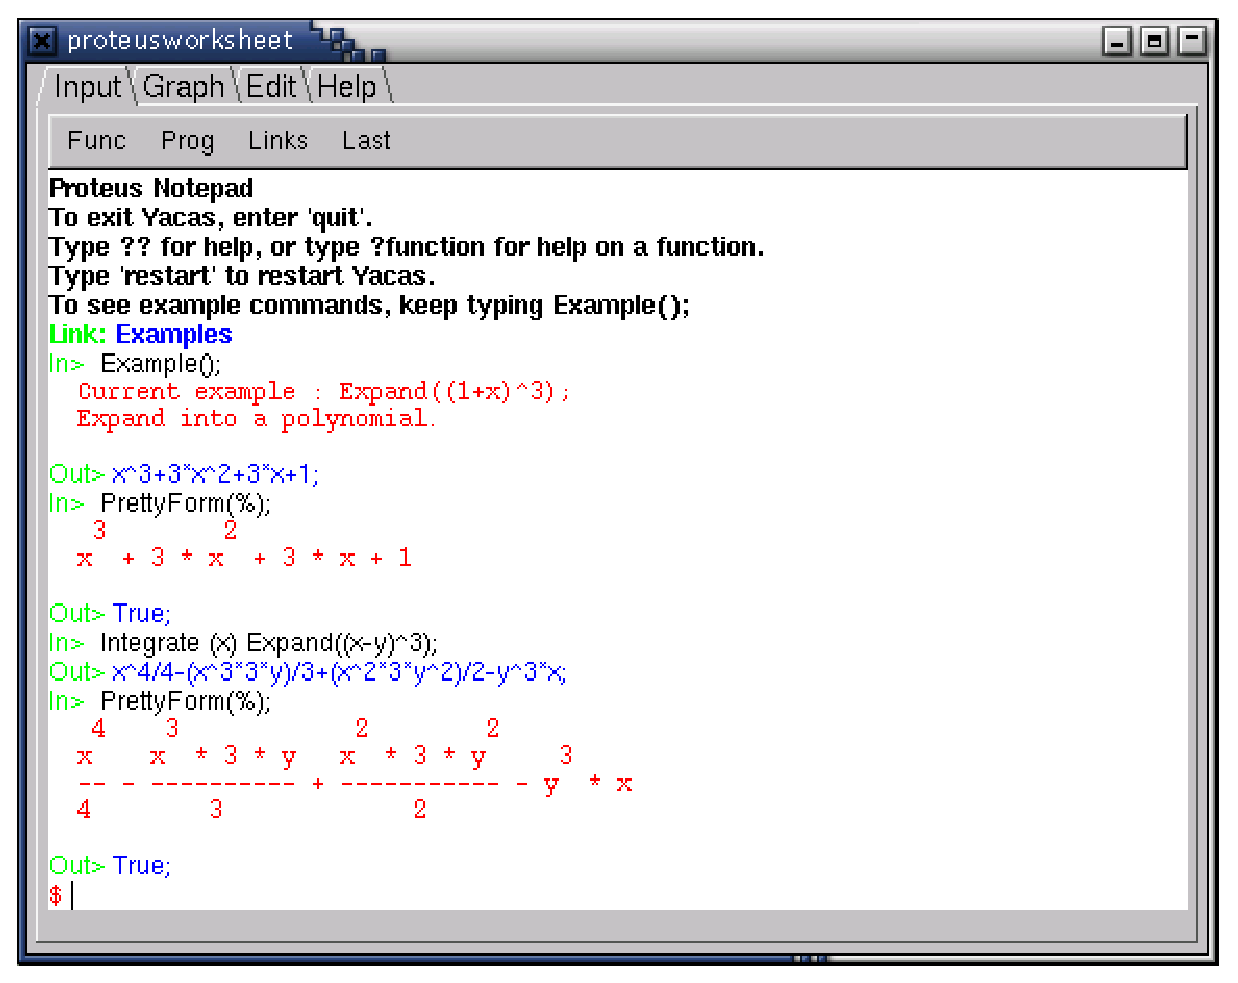
\includegraphics[width=0.65\textwidth]{imagenes/proteus.eps}
%\caption{Proteus, interfaz gráfica para Yacas}
%\end{figure}

%\subsubsection*{Kwordtrans}

%\subsection{Sistema}
%\subsubsection*{gmemusage}
%\subsubsection*{gr_monitor}

%\subsection{Aplicaciones en general}
%\subsubsection*{Creación de CD's}
%\paragraph*{GCombust}
%\paragraph*{XCDRoad?}
%\paragraph*{KreateCD}
%\paragraph*{Kover}

%\subsubsection*{Por Definir}

%% Segunda sección
% \section{Aplicaciones no Gráficas}

% Se  puede  afirmar  que  por cada  aplicación  gráfica  disponible  en
% Linux,  tenemos 50  utilidades  disponibles desde  la terminal.  Estas
% aplicaciones son  el verdadero motor  de todos los  sistemas derivados
% de  UNIX. Con  ellas  se  pueden llevar  a  cabo  infinidad de  tareas
% importantes, desde ordenar  cualquier tipo de archivo  de datos, hasta
% programar  el  encendido  de  una cafetera  para  cuando  nos  estemos
% quedando dormidos. Todas ellas pueden  ser lanzadas desde una terminal
% en modo gráfico, de manera que también las podemos utilizar desde este
% entorno.

%\subsection{Desarrollo}
%\subsubsection*{GCC}
%\subsubsection*{make}
%\subsubsection*{gettext}

%\subsection{Editores}
%\subsubsection*{emacs}
%\subsubsection*{vim}

%\subsection{Gráficos}
%\subsubsection*{ImageMagick}
%\subsubsection*{Otros Filtros}

%\subsection{Internet}
%\subsubsection*{iptraf}
%\subsubsection*{ntop}

%\subsubsection*{aumix}
%\subsubsection*{zgv}
%\subsubsection*{aatv}

%\subsection{Ofimática}
%\subsubsection*{bc}
%\subsubsection*{}

%\subsection{Sistema}
%\subsubsection*{top}
%\subsubsection*{crontab}
%\subsubsection*{at}
%\subsubsection*{uptime}
